
\section{Experiments}

\subsection{Data Collection}

In order to semantically transfer similar expressions from one texture to another, the training data must be collected in a way so that 
corresponding expression textures across different individuals are aligned.  To do this, we hired actors to perform a series of 21 expressions based on the Facial Action Coding System (FACS) ~\cite{Ekman:1978}, and recite 20 Harvard Sentences ~\cite{HarvardSent:1969}. We then hand cut, warped, and aligned the sequences using video editors.  Each FACS expression was broken
up and extended into two 24-frame sequences.  The first of these consisted of an individual starting on neutral frame, then moving to the apex of the FACS expression.
The second 24-frame sequence was a different clip of the face starting in the FACS expression and returning to neutral.  The sentences were aligned
using dynamic time warping on the audio sequences to align the video sequences, as was done in ~\cite{olszewski2016high}. We plan to release this synchronized, high-resolution dataset to the public in the future. 

After aligning the sequences, we used a face-tracking and texture extraction process based on the formulation of ~\cite{f2f}, to compute a texture
for each of the aligned video frames.  Our total training dataset consists of a set of 15 identities, each with 3107 frames.

\subsection{Data Augmentation}
In order to increase the generalization ability of our network to subjects whose appearance varies significantly from those in this dataset, we augment it by altering the skin tones of the captured textures. Specifically, we extract lighting-independent and expression-free albedos from the texture images.
We then perform PCA on the albedo images. To each albedo image, we add multiples of the found principal components with magnitudes proportional to the corresponding eigenvalues multiplied with a random variable drawn from a Gaussian with mean zero and standard deviation 0.1. This results in a new series of albedo images that differ from the original in their skin tone and local details.

These albedo textures, combined with the unmodified captured albedo textures, are used as the training data for our network. We generate 15 additonal albedo textures from each of the 15 subjects, giving us a total of 745,680 training images.

\subsection{Training and Testing}

\begin{figure}[h!]
\setlength\tabcolsep{1.5pt}
\centering
\begin{tabular}{cc}

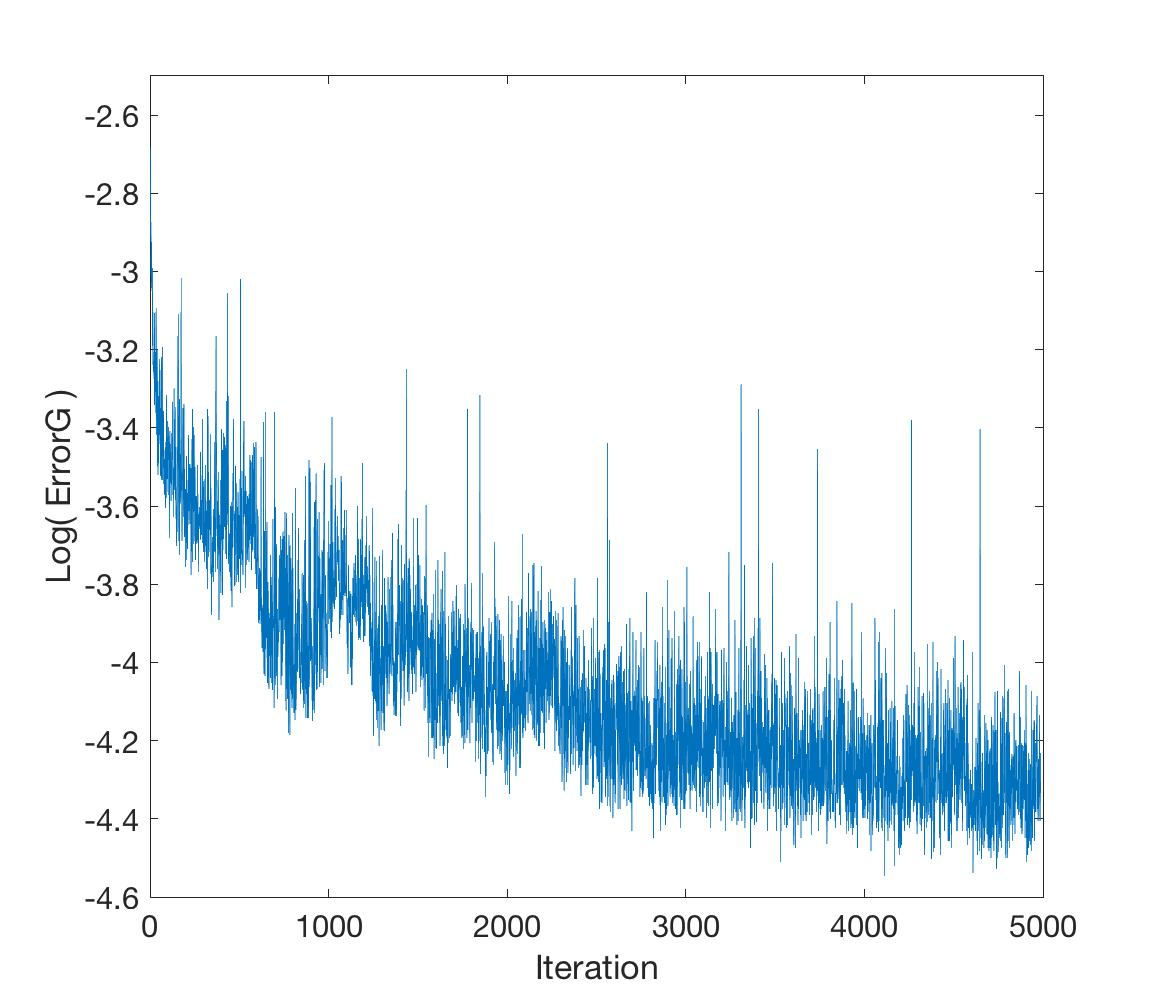
\includegraphics[width=.22\textwidth]{figures/loss/ErrorG2.jpg}&
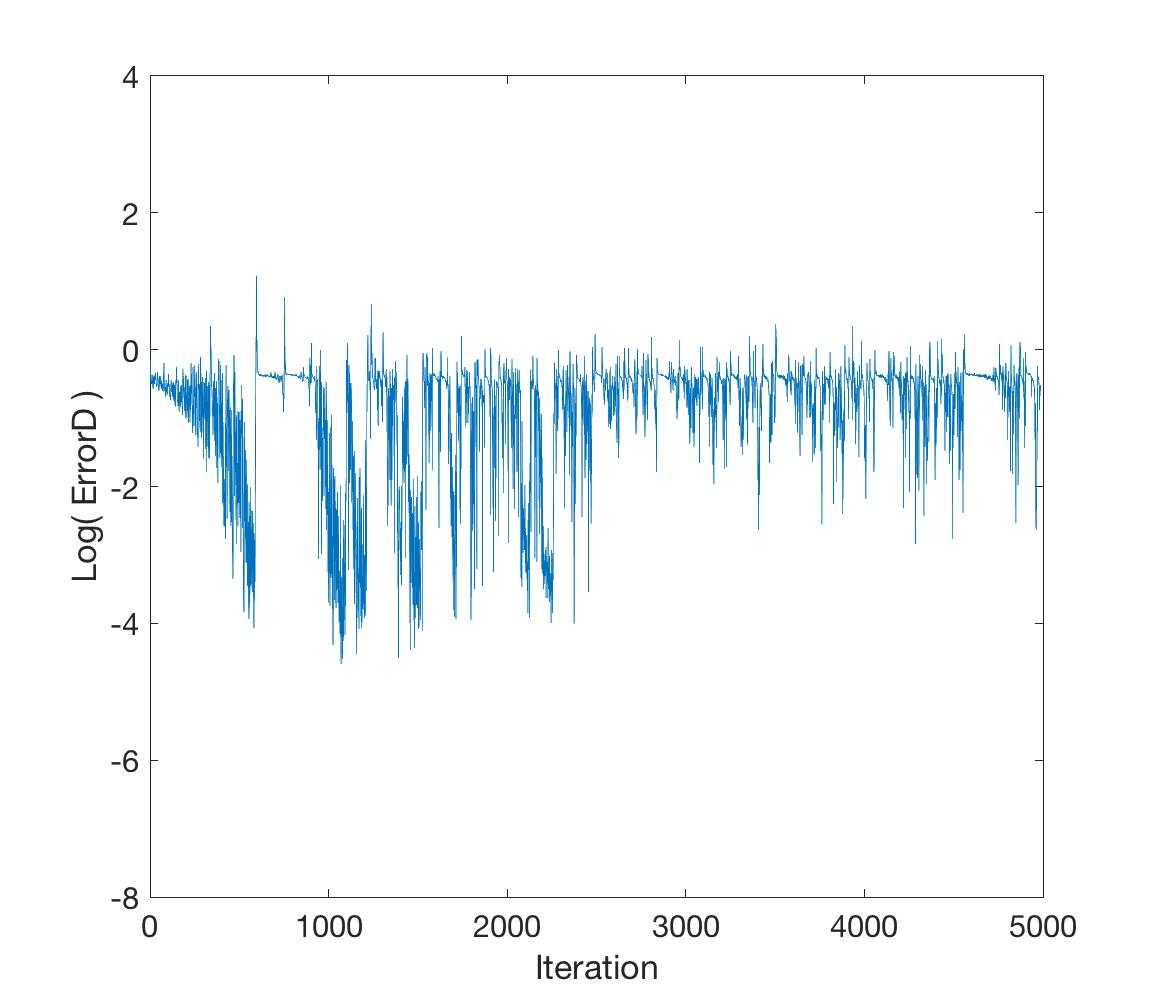
\includegraphics[width=.22\textwidth]{figures/loss/ErrorD2.jpg} \\
Generator Error & Discriminator Error \\ 
\end{tabular}
\caption{Generative and discriminative training loss.}\label{fig:error}
\vspace{-0.05in}
\end{figure} 



We divide the dataset into a training set and a testing set. During training, we train the network in an end-to-end fashion. On each iteration, we randomly sample a pair consisting of a source expression frame and a target identity frame from the dataset as input. The corresponding ground truth texture combining the given identity and expression is also sampled. The output will be synthesized using a forward pass, and the loss is back-propagated using Adaptive Moment Estimation (ADAM). The images are scaled to $256 \times 256$ and we set each batch to contain 64 images. We trained the networks on a Titan X GPU until both the generative loss and discriminative loss converged, which took roughly two days (Fig.~\ref{fig:error}). We set the initial learning rate to $lr=2e-4$ for the generator and $lr=2e-5$ for the discriminator. The learning rate is lowered several times during training. During testing, we randomly sample a pair consisting of a source expression frame and a target identity frame from the test set.
